\section{Software Architecture}

\begin{figure}
\centering
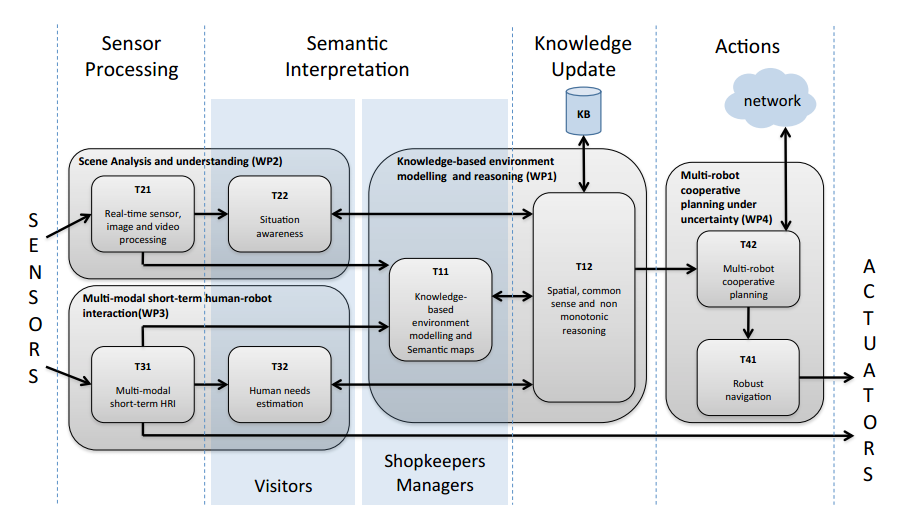
\includegraphics[width=0.95\textwidth]{fig/COACHES_swarch.png}
\caption{COACHES software architecture}
\label{fig:swarch}
\end{figure}

The software architecture of the COACHES robots is shown in Figure \ref{fig:swarch}).
An open architecture (hard/soft) and standard technologies available will be used, 
so that it will be easy to extend and/or adapt the capabilities of the system during the whole length of 
the  project  (especially  to  integrate  and  test  various  algorithms  and/or  sensors).  
Such an open architecture will also simplify and optimize integration efficiency as well as re-use of assets in other projects or products. 


For the development of the software robotics components, the Robot Operating System (ROS)\footnote{www.ros.org}, which is the standard middleware for robotics applications, has been selected.
ROS provides the middleware infrastructure to effectively share information among the many modules implementing various functionalities on each robot. Moreover, an interface (ROS-through-TCP) will be realized in order to share information among the robots and between each robot and other components of the system.

The main software components that will be developed for control, reasoning and interaction functionalities of the system are listed below.

\begin{itemize}
\item T1.1 KB modeling
\item T1.2 KB reasoning
\item T2.1 Image Processing
\item T2.2 Situation Awareness
\item T3.1 Multimodal HRI
\item T3.2 Human needs estimation
\item T4.1 Robust navigation %(Sapienza)
\item T4.2 Multi-robot planning
\end{itemize}

In the next section we will detail the components where Artificial Intelligence techniques have a fundamental role.



